\chapter{Functional programming and computational effects at scale}
~\label{cpt-effects}

This chapter presents and discusses ``Student's Big Brother'' --- a distributed
system to support study workflow in a programming class. It was designed to help
teachers to distribute their attention to all students uniformly. The system consists
of client daemons, watching students activity and sending their source code to a server (over HTTP),
for storage, processing and displaying in teacher web"/interface.
The source code is freely available on GitHub~\cite{sbbRepo}.

The system is mostly implemented using Haskell programming language and the implementation
extensively uses monad transformers and algebraic effects --- the concepts discussed previously
in this thesis --- to structure the necessary side"/effects and separate the effectful
functionality from the pure code.

The rest of the chapter is structured as follows: the first section gives a short
note on motivation for the system's creation; the second section abstractly describes
the system's architecture; the third section focuses on implementation details:
configuration files, integration and deployment and benefits of the use of functional
programming; the last section reports the system usage in real"/life teaching.

\section{Motivation}

It is unfortunate, but most undergraduate students hesitate to ask questions during
programming practice sessions. Usually, the instructing teacher is fighting
students' shyness by walking around the room, observing students and trying to
determine whether the particular student is succeeding or not. But due to the
limited time of the sessions and the fact that there is only one instructor per
10"/15 students, the described procedure is quite inefficient. To approach the
problem, we propose to build a monitoring system for students activities during
programming classes. This system should have features of basic
version control and of displaying the students' source code in a lightweight
web"/interface for the instructor to be able to observe the activity of every
student in real"/time.

The primary purpose of the system is to distribute teachers attention between
all the active students uniformly and to help the teacher to determine which one
needs an assistance but hesitates to ask for it.

\section{System's architecture}

\usetikzlibrary{shapes, arrows, calc, positioning}

\tikzset{
    module/.style={
           rectangle,
           rounded corners,
           draw=black, very thick,
           minimum height=2em,
           inner sep=2pt,
           text centered,
           },
}


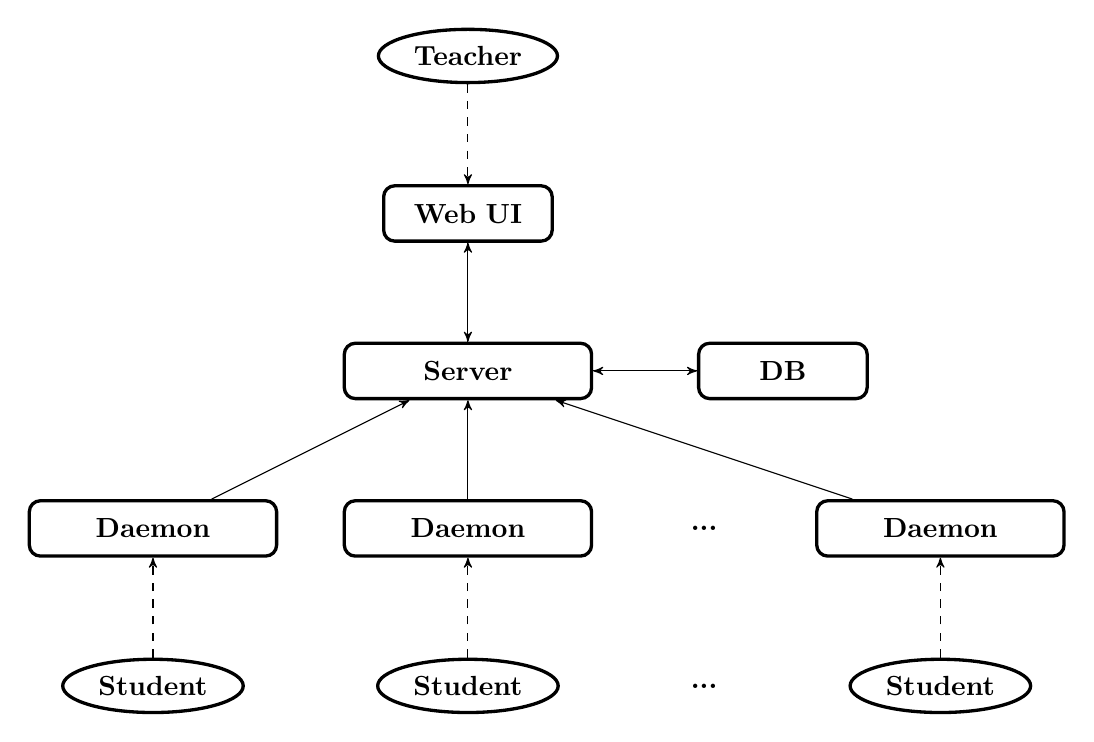
\begin{tikzpicture}[->,>=stealth']

 \node[ellipse, draw=black, very thick] (TEACHER)
 {%
  \textbf{Teacher}
 };

 \node[module,
  yshift=-1cm,
  text width=2cm,
  below of=TEACHER] (UI)
 {%
  \textbf{Web UI}
 };

 \node[module,
  text width=3cm,
  yshift=-1cm,
  below of=UI] (SERVER)
 {%
  \textbf{Server}\\
 };

 \node[module,
  below of=SERVER,
  yshift=-1cm,
  xshift=-4cm,
  anchor=center,
  text width=3cm] (DAEMON_1)
 {%
  \textbf{Daemon}
 };

 \node[module,
  right of=DAEMON_1,
  xshift=3cm,
  text width=3cm] (DAEMON_2)
 {%
  \textbf{Daemon}
 };

 \node[module,
  right of=DAEMON_2,
  xshift=2cm,
  draw=none,
  text width=1cm] (HIDDEN_DAEMONS)
 {%
  \textbf{...}
 };

  \node[module,
  right of=HIDDEN_DAEMONS,
  xshift=2cm,
  text width=3cm] (DAEMON_3)
 {%
  \textbf{Daemon}
 };

 \node[module,
  right of=SERVER,
  xshift=3cm,
  text width=2cm] (DB)
 {%
  \textbf{DB}
 };

 \node[ellipse, draw=black, very thick,
       below of=DAEMON_1,
       yshift=-1cm, ] (STUDENT_1)
 {%
  \textbf{Student}
 };

  \node[ellipse, draw=black, very thick,
       below of=DAEMON_2,
       yshift=-1cm, ] (STUDENT_2)
 {%
  \textbf{Student}
 };

  \node[ellipse,
       below of=HIDDEN_DAEMONS,
       yshift=-1cm, ] (HIDDNE_STUDENT)
 {%
  \textbf{...}
 };

  \node[ellipse, draw=black, very thick,
       below of=DAEMON_3,
       yshift=-1cm, ] (STUDENT_3)
 {%
  \textbf{Student}
 };

 \path (DAEMON_1) edge (SERVER);
 \path (DAEMON_2) edge (SERVER);
 \path (DAEMON_3) edge (SERVER);

 \path (SERVER) edge (DB);
 \path (DB) edge (SERVER);

 \path (SERVER) edge (UI);
 \path (UI) edge (SERVER);

 \path (TEACHER) edge[dashed] (UI);

 \path (STUDENT_1) edge[dashed] (DAEMON_1);
 \path (STUDENT_2) edge[dashed] (DAEMON_2);
 \path (STUDENT_3) edge[dashed] (DAEMON_3);

\end{tikzpicture}

The system consists of three software components: the server, the client daemon and the
teacher's web user interface (UI). The communication between all participants is performed
over HTTP using JSON"/formatted messages.

The rest of this section gives a more detailed account of the role of every component.

\subsection{Daemon: data collection agent}

The client daemon is a data collection agent. It is designed to run silently on
a student's computer, observe student's activity and report it to a server.

The daemon's operation protocol is simple: it runs on a student's computer,
watches the working directory for changes in source code files and regularly sends
these changes to the application server for storage and distribution.

\subsection{Server: data keeper and distributor}

The server's role is to be the central authority for the daemons: collect the files
the send, store them in a database and give them to the web UI on demand.

The server's code is essentially a CRUD"/service~\cite{Martin:1983:MDB:538746} ---
it implements creation, removing, updating and deletion procedures of the considered
entities --- source code files  --- and maps these operations onto database procedures.

\subsection{Web UI: data presenter}

The web UI conveys the information about current state of students works to the teacher.
It keeps up with the present state of server's database and provides a minimalistic
interface to browse the files of every student separately.

\section{Implementation details}

The server and the client daemon are implemented with Haskell programming language
and employ Haskell's type system to enforce safety and correctness of operation
and communication. The teacher's web application is built with standard web stack:
HTML, CSS and JavaScript.

\subsection{Type"/safe communication: sharing types between client and server}

\subsection{Extensible effects at daemon's service}

\section{Exploitation experience report}

The experiment of integration of the developed system into the teaching workflow
of an undergraduate programming course in I.~I.~Vorovich institute of mathematics,
mechanics and computer science was successful. A teacher who has been leading the
class reported the system to be reliable and the user experience to be satisfying.
It was also reported that students had been showing more effort to complete the
tasks and their hesitation for asking questions have been significantly reduced.
